\chapter{Neuroscience}

\section{Neurons}

\section{Neural Circuits}

\subsection{Retinal Circuits}


\subsection{Neocortical Circuits}

A review of various experimental findings on cortical circuits is presented in \cite{harris2015neocortical}. While there are differences in cortical structure and activity across different areas and species, many cortical circuit properties are conserved. \cite{harris2015neocortical} therefore argues that these differences are \textit{quantitative} rather than \textit{qualitative}, arising from differences in gene expression and inputs. They refer to these slight differences on a main conserved architecture as \textit{serial homology}. The primary categorization of neocortical neurons is between excitatory cells (EC), which constitute roughly $80\%$ of neurons, and interneurons, which constitute the remaining $20\%$.  

A somewhat more simplistic view, with a focus on predictive coding, is presented in \cite{bastos2012canonical}.

\subsubsection{Excitatory Cells}

Excitatory cells are classified into three main categories:
\begin{itemize}
	\item \textbf{intratelencephalic (IT) neurons}: Found in layers 2-6 and project axons only within the telecephalon (neocortex, striatum, and corticoid structures such as amygdala and claustrum). They are the only ECs that project to contralateral cortex. There are many distinct subclasses of IT cells, such as those found in L4.
	\item \textbf{pyramidal tract (PT) neurons}: These are large pyramidal neurons found in layer 5B that project to subcerebral targets including brain stem, spinal cord and midbrain, as well as thalamus and striatum. 
	\item \textbf{corticothalamic (CT) neurons}: Found in layer 6 and project primarily to ipsilateral thalamus.
\end{itemize}
Morphologies of these cell types are shown in Figure \ref{fig: cortical morphologies}. It should be noted that all class of ECs form recurrent connections with local neurons of the same class. Across classes, however, the connectivity is asymmetric, which has led to the hypothesis of a sequential circuit organization. This sequence is typically understood in terms of
$$ \text{thalamus} \rightarrow \text{L4 IT neurons} \rightarrow \text{Other IT neurons} \rightarrow \text{PT neurons},$$
with the role of CT neurons within the circuit still largely unknown. 

\begin{figure}[h]
    \centering
    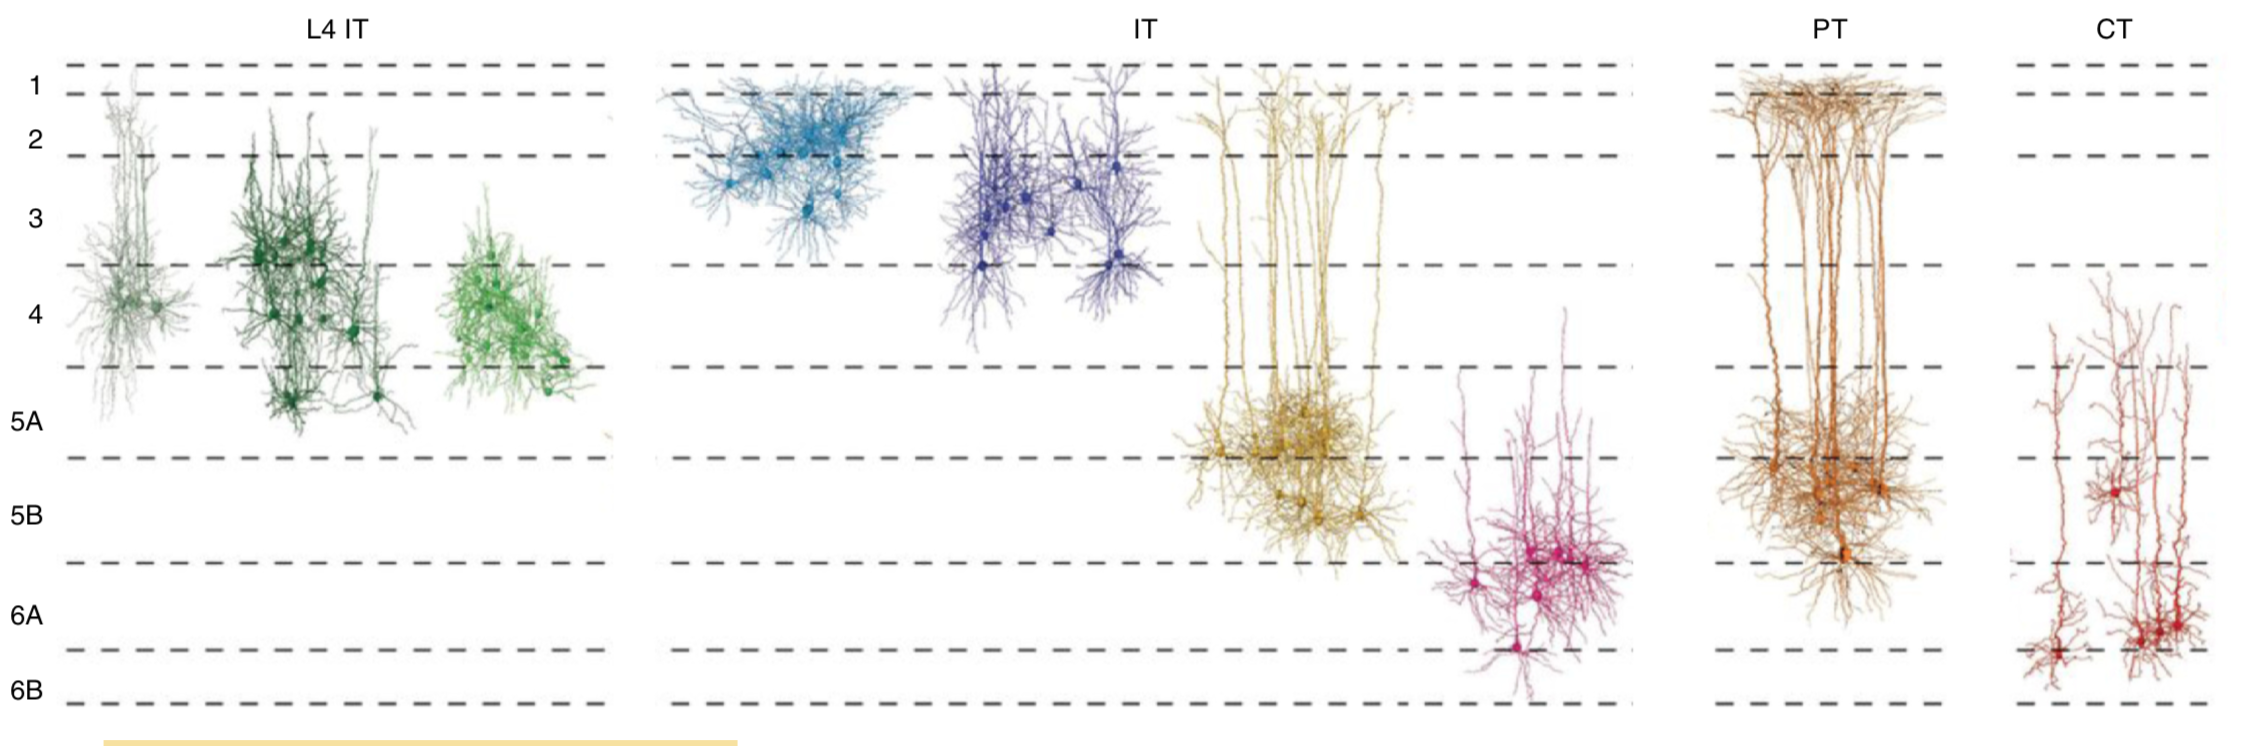
\includegraphics[width=\textwidth]{images/neuroscience/cortical_morphologies.png}
    \caption{Morphologies of various classes of excitatory cells in neocortex. Reproduced from \cite{harris2015neocortical}.}
    \label{fig: cortical morphologies}
\end{figure}

Most of the subcortical inputs to the cortex arise from thalamus and are roughly divided into ``core" and ``matrix" connections. The core relay neurons carry rapid sensory or motor information and are located in primary relay nuclei. These axons tend to form topographic connections in L4 or primary sensory areas. The matrix relay neurons are not well understood, but are typically found in higher order nuclei and project to L1 (and sometimes other layers) of one or more cortical areas. The core-matrix distinction applies most directly to primary sensory areas, but is also found in motor areas and possibly other areas. Higher order sensory cortex, for instance, receives predominantly matrix-type thalamocortical (TC) connections. 

L4 neurons are a special case of IT neurons. They project asymmetrically to L2/3 and L5, and are therefore considered ``upstream" of other circuit components. There are many morphological subclasses of L4 IT neurons, but they largely have similar circuit properties. Layer 4 is enlarged in primary sensory areas, so L4 neurons are thought to be specialized for sensory processing, with different sensory areas tuned appropriately. In higher-order sensory areas, L4 receives input from thalamus as well as lower areas of cortex. Although motor areas appear to lack a well defined L4, they may contain L4 type cells. 

Other IT neurons receive input from L4 neurons and TC connections. Their outputs project to distant neocortical and striatum areas as well as locally to PT and CT neurons. L2 IT neurons receive matrix-type TC input and inputs from L5A and L4. L3 IT neurons receive similar inputs, with the addition of core-type TC inputs. These neurons tend to exhibit sparse firing and project to L5. The L5 IT neurons tend to be reciprocally connected to L2/3 and also have broad range connections, particularly to striatum. L6 IT neurons are less studied but tend to make distant connections. 

PT neurons receive cortical (L2/3) and TC (core-type) input and project to specialized subcortical areas, such as spinal or tectal areas. They also make connections with ipsilateral cortex and thalamus. They tend to display bursting firing patterns, which provide a ``dense code." This is perhaps an information-theoretic adaptation to broadcast cortical output through a small number of channels. 

CT neurons are found in L6, and tend to receive input from higher-order cortical areas, as well as some input from thalamus. Their projections to thalamic areas are slow and weak, so they are often considered as modulators instead of drivers. It is thought that CT neurons may integrate long-range cortical inputs to modulate TC activity, acting as a sort of gain control. 

\begin{figure}[h]
    \centering
    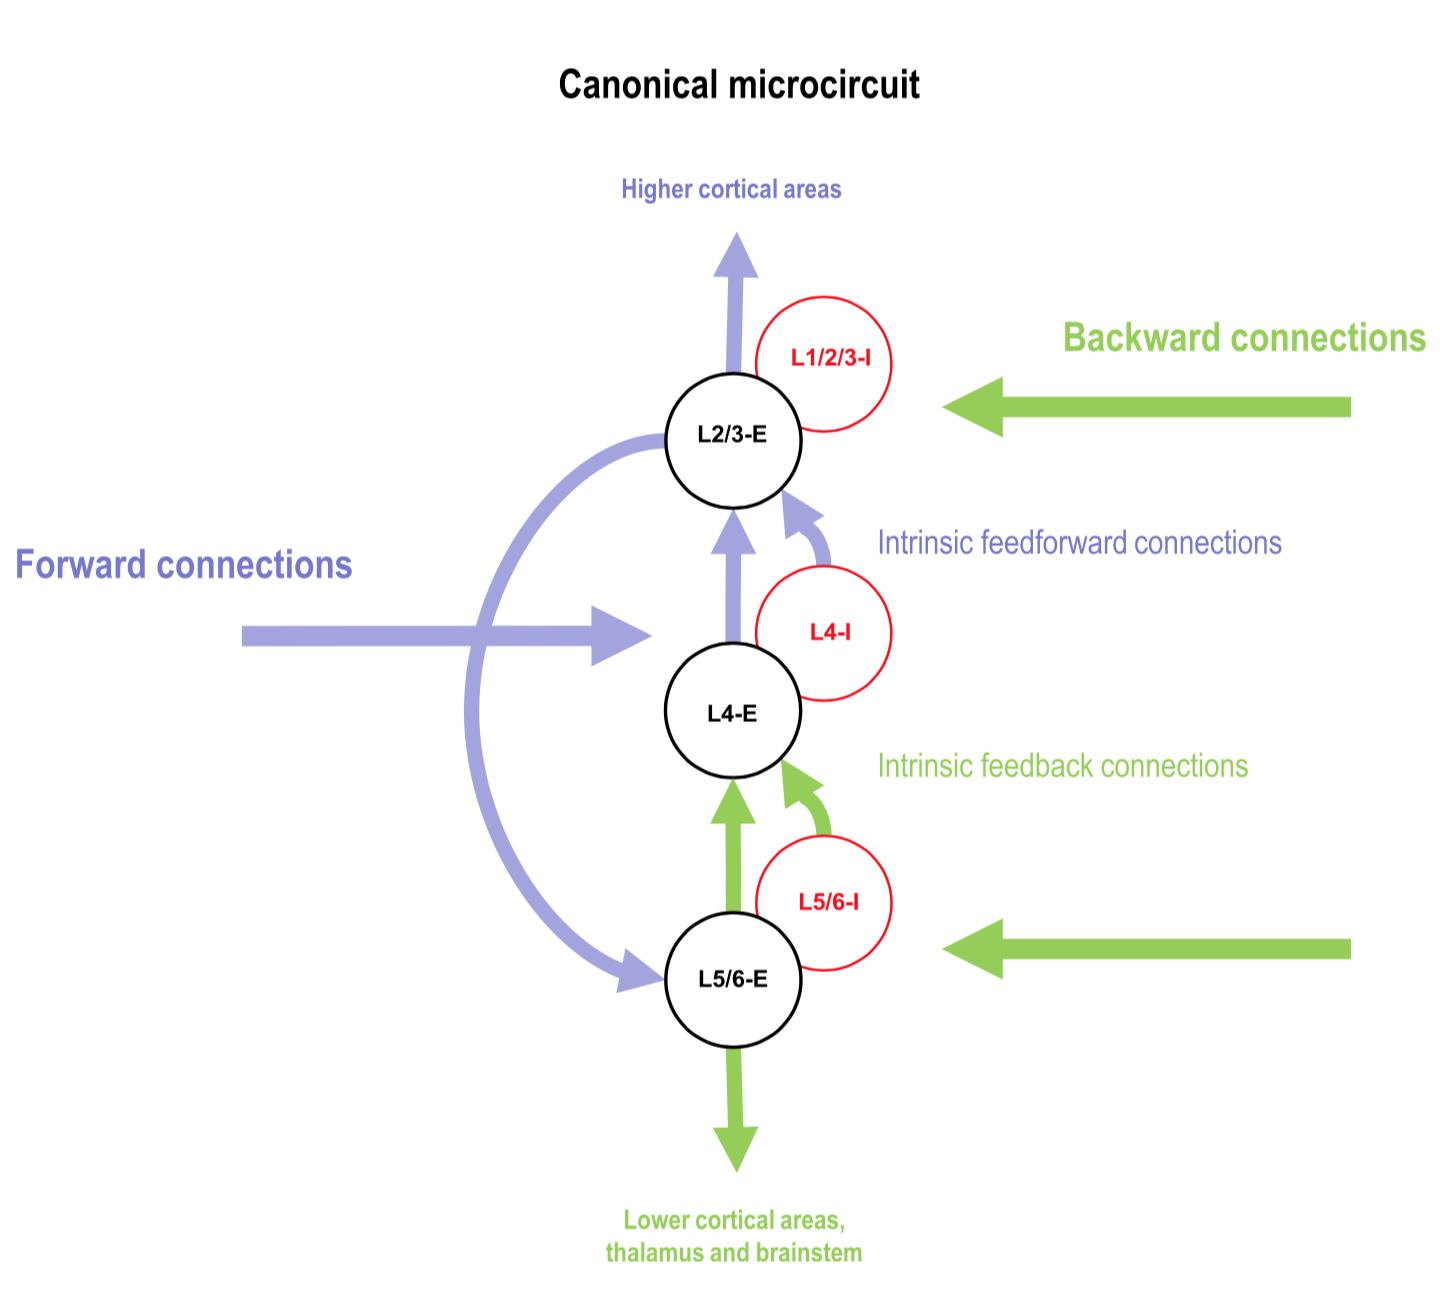
\includegraphics[width=0.75\textwidth]{images/neuroscience/pc_connectivity.png}
    \caption{Connectivity diagram for a cortical microcircuit. Reproduced from \cite{bastos2012canonical}.}
    \label{fig: pc connectivity}
\end{figure}

\subsubsection{Interneurons}

Cortical interneurons are categorized into three classes based on gene expression:
\begin{itemize}
	\item \textbf{Pvalb}
	\item \textbf{Sst}
	\item \textbf{Htr3a}
\end{itemize}
Interneurons contain many subclasses, which inhibit various local ECs and other interneurons. These inhibitory circuits may mediate diverse control of cortical processing during behavior, at least partially contributing to the quantitative differences between cortical circuits that perform different computations, yet have similar qualitative architectures. 


\section{Brain Structures}

\section{Canonical Neural Computations}

\subsection{Linear Weighting}


\subsection{Exponentiation}


\subsection{Normalization}

\cite{carandini2012normalization} reviews various forms of normalization that appear in different brain areas and species. They define (divisive) normalization as \textit{the computation in which the responses of neurons are divided by a common factor that typically includes the summed activity of a pool of neurons}. They point to examples of normalization in olfactory pathways, retinal contrast adaptation, V1, MT, V4, IT, medial superior temporal area (MST), auditory cortex, and lateral intraparietal area (LIP). They also point to a role of normalization in mediating attentional mechanisms, such as winner-take-all competition. The authors offer a number of reasons for the ubiquity of normalization, i.e. possible uses:
\begin{itemize}
	\item \textbf{Maximizing Sensitivity}: adjusting the gain of neural responses to stay within the dynamic range.
	\item \textbf{Invariance}: discarding mean activation information and various irrelevant features
	\item \textbf{Neural Decoding}: treating a population of neurons as a normalized probability distribution
	\item \textbf{Stimuli Discrimination}: making discrimination easier for a linear classifier
	\item \textbf{Max Pooling}: biased and winner-take-all competition
	\item \textbf{Redundancy Reduction}: increasing the efficiency of neural representations by creating statistically independent activations.
\end{itemize}
Normalization is implemented in various circuits using various biophysical mechanisms, such as inhibition (polarization modulation), shunting inhibition (conductance modulation), and synaptic depression. Across many implementations, the overall computational scheme appears to rely on a ``summation field" and a ``suppression field," in which the activity of the summation field is divisively normalized according to the suppression field.